%%%%%%%%%%%%%%%%%%%%%%%%%%%%%%%%%%%%%%%%%
% Thin Sectioned Essay
% LaTeX Template
% Version 1.0 (3/8/13)
%
% This template has been downloaded from:
% http://www.LaTeXTemplates.com
%
% Original Author:
% Nicolas Diaz (nsdiaz@uc.cl) with extensive modifications by:
% Vel (vel@latextemplates.com)
%
% License:
% CC BY-NC-SA 3.0 (http://creativecommons.org/licenses/by-nc-sa/3.0/)
%
%%%%%%%%%%%%%%%%%%%%%%%%%%%%%%%%%%%%%%%%%

%----------------------------------------------------------------------------------------
%	PACKAGES AND OTHER DOCUMENT CONFIGURATIONS
%----------------------------------------------------------------------------------------

\documentclass[a4paper, 12pt]{article} % Font size (can be 10pt, 11pt or 12pt) and paper size (remove a4paper for US letter paper)

\usepackage[protrusion=true,expansion=true]{microtype} % Better typography
\usepackage{graphicx} % Required for including pictures
\usepackage[utf8]{inputenc}
\usepackage[margin=1.0in]{geometry}
\usepackage{url}
\usepackage{fancyhdr}
\usepackage{amsmath}
\usepackage{setspace}
\usepackage{enumitem}
\setlength\parindent{0pt} % Removes all indentation from paragraphs

\usepackage[T1]{fontenc} % Required for accented characters
\usepackage{times} % Use the Palatino font

\usepackage{listings}
\usepackage{color}
\lstset{mathescape}

\definecolor{dkgreen}{rgb}{0,0.6,0}
\definecolor{gray}{rgb}{0.5,0.5,0.5}
\definecolor{mauve}{rgb}{0.58,0,0.82}

\lstset{frame=tb,
   language=c++,
   aboveskip=3mm,
   belowskip=3mm,
   showstringspaces=false,
   columns=flexible,
   basicstyle={\small\ttfamily},
   numbers=none,
   numberstyle=\tiny\color{gray},
   keywordstyle=\color{blue},
   commentstyle=\color{dkgreen},
   stringstyle=\color{mauve},
   breaklines=true,
   breakatwhitespace=true
   tabsize=3
}
\linespread{1.00} % Change line spacing here, Palatino benefits from a slight increase by default

\makeatletter
\renewcommand{\@listI}{\itemsep=0pt} % Reduce the space between items in the itemize and enumerate environments and the bibliography

\renewcommand\abstractname{Résumé}
\renewcommand\refname{Références}
\renewcommand\contentsname{Table des matières}
\renewcommand{\maketitle}{ % Customize the title - do not edit title and author name here, see the TITLE block below
\begin{center} % Right align

\vspace*{25pt} % Some vertical space between the title and author name
{\LARGE\@title} % Increase the font size of the title

\vspace{125pt} % Some vertical space between the title and author name

{\large\@author} % Author name

\vspace{125pt} % Some vertical space between the author block and abstract
Dans le cadre du cours
\\INF8702 - Infographie avancée
\vspace{125pt} % Some vertical space between the author block and abstract
\\\@date % Date
\vspace{125pt} % Some vertical space between the author block and abstract

\end{center}
}

%----------------------------------------------------------------------------------------
%	TITLE
%----------------------------------------------------------------------------------------

\title{TP1 : ShaderGen} 

\author{\textsc{Guillaume Arruda 1635805\\Raphael Lapierre 1644671} % Author
\vspace{10pt}
\\{\textit{École polytechnique de Montréal}}} % Institution

\date{18 Septembre 2015} % Date

%----------------------------------------------------------------------------------------

\begin{document}

\thispagestyle{empty}
\clearpage\maketitle % Print the title section
\pagebreak[4]
%----------------------------------------------------------------------------------------
%	En tête et pieds de page 
%----------------------------------------------------------------------------------------

\setlength{\headheight}{15.0pt}
\pagestyle{fancy}
\fancyhead[L]{INF8702}
\fancyhead[C]{}
\fancyhead[R]{TP1 - ShaderGen}
\fancyfoot[C]{\textbf{page \thepage}}

%----------------------------------------------------------------------------------------
%	ESSAY BODY
%----------------------------------------------------------------------------------------
\section*{Implémentation}

\section*{Questions}

\subsection*{Votre nuanceur de sommets fait appel à la fonction "ftransform()"}
\begin{description}[style=nextline]
    \item[Que fait cette fonction?]
        La fonction \textit{ftransform()} permet de transformer un vertex en coordonnées
        local (\textit{model}) à une position de projection sur l'écran. On peut voir la fonction
        comme l'équivalent d'appeler $v = gl\_ProjectionMatrix * gl\_ModelViewMatrix *
        gl\_Vertex $.
    \item[Que fait alors la fonction fnormal()?]
        La fonction \textit{fnormal()} permet de transformer le vecteur normal d'un vertex
        en coordonnées local à celles de la camera. Elle utilise une matrice particulière
        qui est la transposée de l'inverse de la \textit{model-view matrix}.
\end{description}

\subsection*{Les fonctions gl\_ModelViewMatrix, gl\_NormalMatrix sont toutes intégrées à 
             l'API(built-in)"}
\begin{description}[style=nextline]
    \item[En faisant référence aux matrices de base d'openGL, comment est composée la matrice
          gl\_ModelViewProjectionMatrix?]
        L'équation formant la composition peut s'écrire comme suit. Il est important
        de noter que la multiplication de matrice n'étant pas commutative, l'ordre est 
        important. \\$gl\_ModelViewProjectionMatrix = gl\_ProjectionMatrix *\\ gl\_ViewMatrix *
        gl\_ModelMatrix$.
    \item[Quel est le contenu de la matrice gl\_NormalMatrix?]
        La matrice est composée de la transposée de l'inverse de la \textit{model-view matrix}.
\end{description}

\subsection*{Dans les calculs d'éclairage du nuanceur de sommets, on ne trouve
             nulle part le calcul d'un "reflectedVP" (rayon, ou angle de réflexion du vecteur
             surface-lumière) dans le calcul de la contribution spéculaire. Quel vecteur 
             calcule-t-on à la place? Dessinez ce vecteur.}

Le vecteur utilisé au lieu du vecteur réfléchie est la bissectrice entre le vecteur partant
de la surface vers la source lumineuse et le vecteur partant de l'oeil à la surface. On l'appel
\textit{Half-Vector}. Le schéma demandé est présenté à la figure \ref{schema}.

\begin{figure}[H]
    \label{schema}
    \centering
        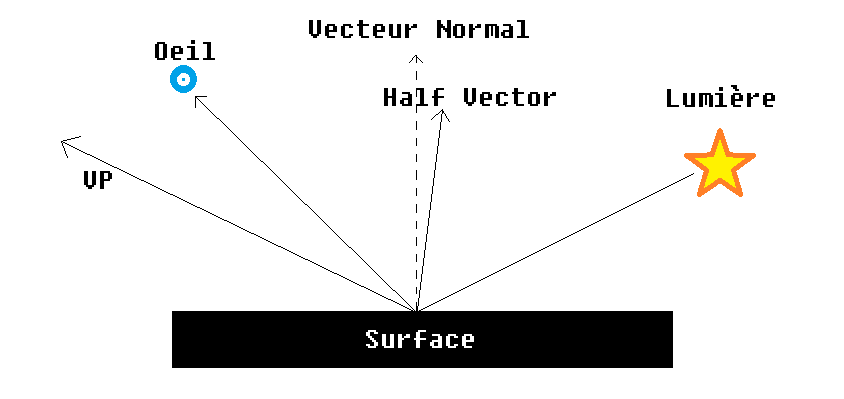
\includegraphics[width=0.75\textwidth]{HalfVector.png}
    \caption{Schéma du \textit{Half-Vector}}
\end{figure}

\subsection*{Cette technique de calcul de la spécularité est celle utilisée dans l'implémentation
             standard d'OpenGL. Ce n'est PAS la technique de Phong. De quelle technique s'agit-il
             (le nom de la personne qui l'a inventée) et expliquez la.}

L'inventeur de la technique s'appel Blinn. Il s'agit en fait d'une modification de la technique
de Phong qui elle utilise le vecteur réfléchie par la surface éclairée. Puisque cette réflection
est couteuse en temps de calcul comparé à la bissectrice donnant le \textit{half-vector}, Blinn
eu l'idée d'utiliser cette dernière plutôt que de calculer la réflexion et remarqua que le 
résultat semblait satisfaisant à l'oeil.

\subsection*{En gros, quelle est la technique à utiliser lorsque l'on veut, au niveau des nuanceurs,
             implémenter la caractérisitique "two-sided lighting"? Expliquez cette technique
             afin d'en démontrer la pertinence/nécessité d'utilisation.}

Pour implémenter la caractéristique \textit{two-sided lighting} on doit effectuer une deuxième
passe de calcul d'éclairage en inversant la normale et en utilisant les couleurs "arrière" du 
matériel. Il est important d'effectuer du \textit{two sided lighting} pour des objets non
fermés sur eux-mêmes sinon leur face de "derrière" semble être totalement noire. Il est pertinent
d'avoir un éclairage fonctionnant de tous les côtés d'un objet lorsque ceux-ci sont visibles.

\subsection*{Dans le nuanceur de fragments, on trouve cette ligne de code : "vec4 texture0Arg0 = 
             texture2D(texUnit0, gl\_TexCoord[0].xy);" Qu'est-ce que le membre ".xy" de 
             gl\_TexCoord[0]?}

Spécifiquement, l'utilisation ".xy" vient du \textit{swizzle} du langage GLSL. À l'aide de celui-ci,
on peut accèder à certains membres d'un vecteur plus facilement. Par exemple, .xy retourne les deux premiers
éléments d'un vecteur. Dans le cas exacte des textures, le membre ".xy" prend les coordonnées uv
spécifiée pour le fragment et va chercher le point qui est associée dans la texture spécifiée.
%----------------------------------------------------------------------------------------
\end{document}
